\documentclass[a4paper,14pt]{article}

\usepackage[utf8]{inputenc}
\usepackage[english]{babel}
\usepackage{graphicx, array, blindtext}
\usepackage[colorinlistoftodos]{todonotes}

\usepackage{enumitem}
\usepackage{amsmath}
\usepackage{amsthm}

\usepackage{nameref}
\usepackage{amssymb}
\usepackage{xcolor}
\usepackage{floatrow}
\usepackage{cancel}
\usepackage{fancyhdr}
\usepackage{graphicx}
\usepackage{verbatim}
\usepackage[document]{ragged2e}

\rhead{CS765 Assignment 2}
\usepackage{subcaption}
\usepackage{listings}


\usepackage{hyperref}

\begin{document}
\centering{

\title{\fontsize{150}{60}{CS765 Assignment 2}}

\author{
Prathamesh Pilkhane\\
Shashwat Garg \\
Vedang Asgaonkar}
}

\date{Spring 2023}
\maketitle

\justifying

% \tableofcontents
% \newpage

\justifying

\section*{Introduction}

Hello and Welcome to our CS765 Project part 2. This builds up on the Blockchain implementation that we developed in the First Assignment.

We introduce adversaries in this part. We incorporate selfish mining and stubborn mining attacks. The report that follows will focus mainly on our implementation of the ideas and then discuss the observations and plots obtained.

\section{Code Flow}

We introduce a new \verb|AttackerNode| class which inherits from the \verb|Node| class. This class holds the private blocks, information about whether it is stubborn/selfish and the current public chain level.

We introduce new functions to initialise and handle these variables specific to the \verb|AttackerNode| and modify the \verb|BroadcastBlockEvent| trigger function to depend on the node type.

The only difference between selfish and stubborn mining is a difference in the transmitting policy upon receiving the block. This is captured in the \verb|_policy()| function.

\section{Observation}

\subsection{MPU Measurements}

We have averaged our measurements over 10 runs of the simulation for different values of the input seeds.

The results are as follows-
\begin{center}
    \begin{tabular}{|c|c|c|}
        \hline
        $MPU_{node_{adv}}$ & Selfish & Stubborn \\
        \hline
        0.25 & 0.075 &	0.295 \\
        0.50 & 0.029 & 0.201 \\
        0.75 & 0.200 & 0.267 \\
        \hline
    \end{tabular}
\end{center}



\begin{center}
    \begin{tabular}{|c|c|c|}
        \hline
        $MPU_{node_{overall}}$ & Selfish & Stubborn \\
        \hline
        0.25 & 0.486 &	0.509 \\
        0.50 & 0.526 & 0.531 \\
        0.75 & 0.526 & 0.545 \\
        \hline
    \end{tabular}
\end{center}


We now perform the same calculations with the attacker having a lot more hashing power. For this particular case, 90\% of the other nodes have low processing power.

\begin{center}
    \begin{tabular}{|c|c|c|}
        \hline
        $MPU_{node_{adv}}$ & Selfish & Stubborn \\
        \hline
        0.25 & 0.443 &	0.642 \\
        0.50 & 0.431 & 0.455 \\
        0.75 & 0.352 & 0.535 \\
        \hline
    \end{tabular}
\end{center}



\begin{center}
    \begin{tabular}{|c|c|c|}
        \hline
        $MPU_{node_{overall}}$ & Selfish & Stubborn \\
        \hline
        0.25 & 0.5 &	0.516 \\
        0.50 & 0.522 & 0.532 \\
        0.75 & 0.5 & 0.537 \\
        \hline
    \end{tabular}
\end{center}

We observe that almost all $MPU_{node_{adv}}$ values increase when we increase the mining power of the attacker. This aligns with expectation and the code also reinforces the idea. We observe that the fraction of attacker blocks in main chain does not match the exact theoretical results, but does follow the trends established in the paper. This can again be attributed to experimental errors and empirical observations.

\subsection{Blockchain Plots}

A sample plot is shown below. In the extreme case shown, for demonstration purposes, it is clear how the attacker has mined a a much longer private chain, though the honest nodes do not see much of it.

\begin{center}
    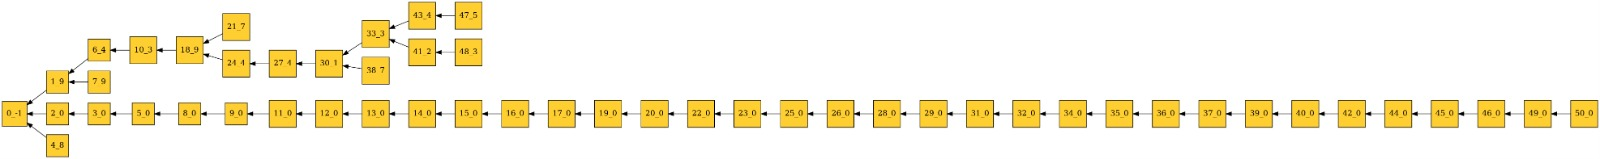
\includegraphics[width=12cm]{attacker.jpeg}\\
    Attacker Node
\end{center}


\begin{center}
    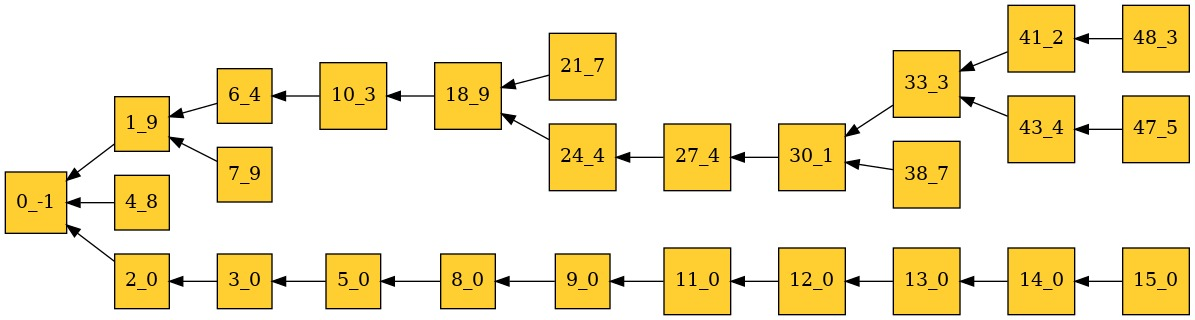
\includegraphics[width=6cm]{normal.jpeg}\\
    Honest Node
\end{center}




\end{document}